% acmtr.tex
% revised 1/20/97
% $Header: acmtr.tex,v 1.5 2/14/96 11:07:57 boyland Exp $

\documentclass[hyperref]{acmtrans2e}
\usepackage{url}
\usepackage{graphicx}
\usepackage{wrapfig}




\graphicspath{ {./images/} }
%&t&{\tt #}&
%&v&\verb|#|&

\newcommand{\BibTeX}{{\rm B\kern-.05em{\sc i\kern-.025em b}\kern-.08em
    T\kern-.1667em\lower.7ex\hbox{E}\kern-.125emX}}

\firstfoot{Detection of cats in images, DTU, June 2015}

\runningfoot{Detection of cats in images, DTU, June 2015}

\markboth{Anna Maria Walach}{Detection of cats in images}

\title{Detection of cats in images}
\author{ANNA MARIA WALACH (s121540) \\Technical University of Denmark\\02238 Biometric Systems}
\begin{abstract}
The \LaTeX\ {\tt acmtrans} document style formats articles in 
the style of the ACM transactions.  Users who have prepared their
document with \LaTeX\ can, with very little effort, produce
camera-ready copy for these journals.  
%Then the ACM production department
%will re-typeset from scratch anyway, introducing typographical errors.
\end{abstract}

\category{D.2.7}{Software Engineering}{Distribution and Main\-ten\-ance}%
[documentation]

\category{H.4.0}{Information Systems Applications}{General}


\terms{Algorithms, Experimentation}

\keywords{cat, detection, images}

\begin{document}

\setcounter{page}{111}

\maketitle

\section{Introduction}
There are more and more projects that uses live streaming and social media power to help and safe feral cats. Some of them are meant to control the population in the area \cite{LAPS:2015}, other focus on raising awareness about feral cats, spaying and neutering importance \cite{TinyKittens:2015} or just to increase changes of finding a new home for homeless cats and kittens \cite{CritterRoom:2015}.
\begin{wrapfigure}[13]{r}{0.5\textwidth}
\centering
    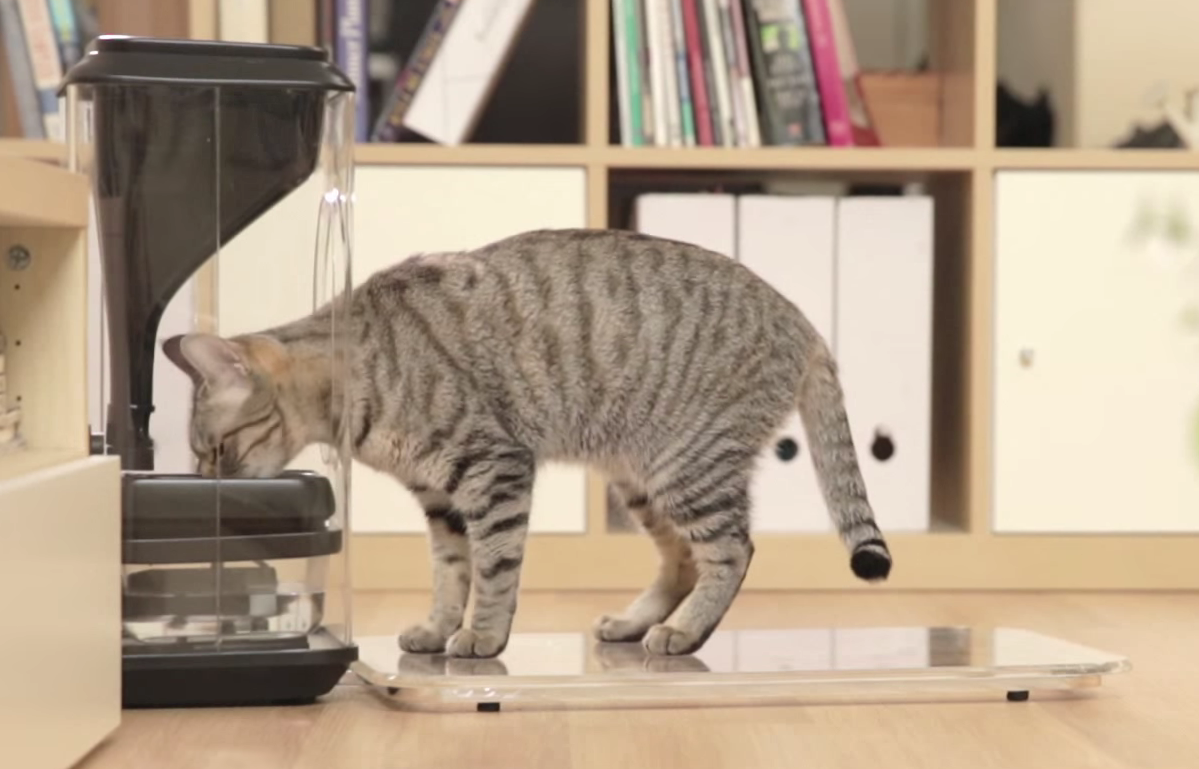
\includegraphics[width=0.48\textwidth]{bistro}
  \caption{CatFi product used by a cat.}
  \label{fig:bistro}
\end{wrapfigure}

People are also more interested in health and safety of their own pets. Lower prices of video technologies and smarthone popularity helped to create various apps for controlling your pet lifestyle. \cite{CatFi:2015} created an automatic feeder with cat identification system and connected it to the smartphone app. It allows owner to supervise the amount of dry food and water his cats are consuming everyday, to receive alarms in case of abnormalities and even spy on them while eating. 

The PiP \cite{PiP:2013} app is designated to help people find their lost cats and dogs. According to American Human Society, almost 3.5 million pets are lost each year and about 80\% of dogs and 98\% of cats are never re-united with their families. The authors of the smarthone app allows the owners to made profiles for their pets (including pictures) and in case the pet is missing, you launch the "alarm" on that pet, together with last seen location. If anyone finds a homeless animal, he may send the photo of it to the PiP app, which automatically try to match one of the lost pets with found pet. 

Increasing number of pets' photographies also encouraged camera producers to implement appropriate support for it in their devices. Right now, Fujifilm company introduced Auto Dog / Cat Detection function \cite{FujiFilm:2009} in some of their cameras that allows to automatically detect pet's face on the image and put auto-focus on it. 
 
\subsection{Problem description}
Almost all of the applications and initiatives described in previous section already use or would benefit from the cats detection and/or identification. In this research I would like to focus on topic of cat detection in images. The main interest is on the use case of detecting cats presence in shots from live cameras and streams. Such images are characterized by  diversified, often bad lighting settings, with possible presence of another animals or human beings. I will perform a comparison of existing solutions and propose own framework that deals with this problem.

\section{The state of the art}
commeercial solutions
\section{Methodology}

\subsection{Overfull hbox - Stretching/filling one horizontal line}

To solve a line break due to ``Overfull \verb|\hbox|'', here is a plain \TeX\ 
solution; here \verb|\hsize| is the default setting of acmtrans.sty:

\begin{center}
\verb|\hbox to \hsize{line sentence to be stretched}|
\end{center}

This can be used in a list environment as well but \verb|\hsize| declared to a reduce
dimension:

\begin{verbatim}
   \hbox{\vbox{\hsize = less than the default setting
   \hbox to \hsize{line sentence to be stretched}}}
\end{verbatim}

\subsection{Programs}

Good formatting of programs requires a knowledge of their semantics,
and is beyond the scope of a document production system.  While
``pretty printers'' are useful for handling the many pages of a real
program, the short examples that are published in articles should be
formatted by hand to improve their clarity.  The \LaTeX\ {\tt tabbing}
environment makes the formatting of programs relatively easy,
especially if the user defines commands for his particular language
constructs.
One may also use the {\tt verbatim} environment.

The ACM transactions style requires that programs be formatted with
different size fonts, depending upon whether they appear in the text or
in a figure, but that is handled by the figure macro which
automatically sets the correct font size.
%The {\tt acmtrans} style provides a {\tt program}
%environment that is exactly the same as the standard {\tt tabbing}
%environment except for the size of the fonts it uses.  This environment
%should be used for formatting programs, whether they appear in the
%running text or in a figure.
Moreover, programs in running text should be indented two ems 
on each side (as provided by the {\tt quote} environment), and
programs in regular figures should be centered.
(Programs in ``narrow figures'' (q.v.) are left or right justified
automatically).

Here is an example of a program:
\begin{quote}
\begin{tabbing}
{\bf type} date =\\
\hspace*{1em}\= {\bf record} \= day: 1\,.\,.\,31;\+\+\\
                                month: 1\,.\,.\,12;\\
                                year: integer \-\\
                {\bf end} \-\\
{\bf var} mybirth, today : date;\\
{\bf var} myage : integer;
\end{tabbing}
\end{quote}
Figure~\ref{fig:prog} shows how the same program looks in a figure.
\begin{figure}
\centerline{\parbox{104pt}{% it's safe to overestimate the size here
\begin{tabbing}
{\bf type} date =\\
\hspace*{1em}\= {\bf record} \= day: 1\,.\,.\,31;\+\+\\
                                month: 1\,.\,.\,12;\\
                                year: integer \-\\
                {\bf end} \-\\
{\bf var} mybirth, today : date;\\
{\bf var} myage : integer;
\end{tabbing}}}
\caption{An example of a program centered in a figure}
\label{fig:prog}
\end{figure}

%The ACM standard calls for the program to start flush at the left
%margin, with each new level of nesting indented by a distance of one
%em, and with the continuation of broken lines indented two ems.  However,
%this standard is not applied consistently.

In addition to formatting programs, the {\tt tabbing} environment may be
used for similar displayed material such as BNF syntax specifications
and rewrite rules.
\section{Figures and Tables}

\subsection{Figures}

The ordinary \LaTeX\ {\tt figure} environment works as usual.
Figure~\ref{fig:ordinary}, which is Figure~6 of \citeN{7:3:359}, a bogus reference,
\begin{figure}
\centering
\(\begin{array}{c|ccc}
     & \bot & F & T \\
\hline
\bot & \bot & \bot & T \\
F    & \bot & F    & T \\
T    & \bot & T    & T
\end{array}\)
\caption{The truth table for the parallel-or.}
\label{fig:ordinary}
\end{figure}
was produced in this way.
Note that figures should never appear in the text or at the bottom of
a page. (If you use the figure placement optional argument, use only
\verb"t" or \verb"p" or both; do not use \verb"h" or \verb"b").

Some figures (and tables) have no caption except for the figure number.
For such figures (and tables), one uses a \verb|\nocaption| command,
which has no argument, instead of the \verb|\caption| command.

In addition to this method of formatting figures, the ACM transactions
also uses figures with side captions, as in Figure~\ref{fig:narrow}.
Such a figure is produced with the {\tt narrowfig} environment.  This
environment has a single mandatory argument, which is the width of the
figure.
Note that if the figure is generated by {\tt tabbing} or {\tt
tabular}, one can safely overestimate the size.
It works just like the ordinary {\tt figure} environment,
except it must contain only one \verb|\caption| or \verb|\nocaption|
command, which must come after the figure itself.  

The {\tt narrowfig} environment should obviously not be used unless the
figure is narrow enough to leave a reasonable amount of space beside it
for the caption.  The ACM seems to have no consistent policy for choosing
which style of figure to employ.

\subsection{Tables}

The ordinary \LaTeX\ {\tt table} environment can be used, but it
requires the user to add formatting commands to match the ACM
transactions style.  This formatting is performed automatically
if the {\tt acmtable} environment is used instead, producing
the result shown in Table~\ref{tab:table}, which shows the same
table displayed in Figure~\ref{fig:ordinary}.
\begin{acmtable}{100pt}
\centering
\(\begin{array}{c|ccc}
     & \bot & F & T \\
\hline
\bot & \bot & \bot & T \\
F    & \bot & F    & T \\
T    & \bot & T    & T
\end{array}\)
\caption{The truth table for the parallel-or.}
\label{tab:table}
\end{acmtable}

\subsection{Bibliography}

\begin{enumerate}
\item{[Cytron et al. 1991]} $\rightarrow$ \verb|\cite{cytron-et-al-toplas91}|
\item{Briggs et al. [1994]} $\rightarrow$ \verb|\citeN{briggs-cooper-torczon-toplas94}| or
\end{enumerate}
\noindent
The list will be updated as we find unique cases.

\bibliographystyle{acmtrans}
\bibliography{acmtr}
\begin{received}
Received February 1986;
November 1993;
accepted January 1996
\end{received}

\end{document}





